\chapter[SYSTEM DESIGN (RESEARCH METHODOLOGY)]{\hfill CHAPTER 3 \hfill\null\vskip15pt SYSTEM DESIGN (RESEARCH METHODOLOGY)}

{\textless}What solutions or techniques are being used?  What technology is current and is it effective?{\textgreater}

\begin{figure}[H]
\centering
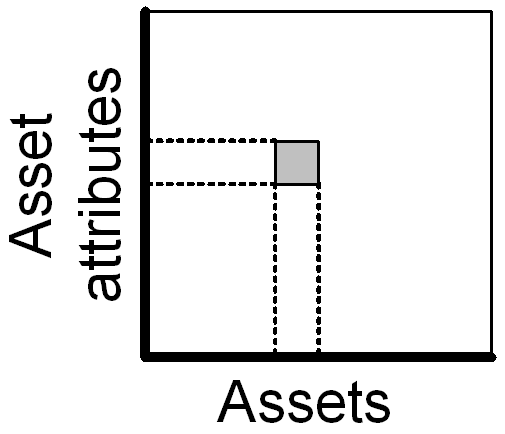
\includegraphics[width=0.25\textwidth]{img/figure1}
\caption{Asset decision sub-space {\textless}sample figure{\textgreater}}\label{fig:1}
\end{figure}
{\textless}Make sure your caption uses the ‘Figure’ style{\textgreater}

\begin{table}[H]
	\centering
	\caption{Software process modeling constructs {\textless}Sample table{\textgreater}}
	\label{tab:01}
	\begin{tabular}{p{0.33\linewidth-2\tabcolsep}p{0.67\linewidth-2\tabcolsep}}
		\toprule
		\multicolumn{1}{c}{\textbf{Modeling construct}} & \multicolumn{1}{c}{\textbf{Description}} \\ \midrule
		Agents & An actor who performs an activity (process element) \\
		Roles & Set of responsibilities assigned to an agent \\
		Artifacts & A product created or maintained by the activities \\
		Activities & Steps that need to achieve process objectives \\
		Tools & Are to be utilizes by the process \\ \bottomrule
	\end{tabular}
\end{table}

{\textless}Make sure your caption uses the ‘Table’ style{\textgreater}